\documentclass[tikz,border=12pt]{standalone}
\usepackage[T1]{fontenc}
\usepackage[utf8]{inputenc}
\usepackage{lmodern}
\usetikzlibrary{calc}

% Tetraedro FSPC — arquivo independente, compilável com pdflatex.
% No pôster, exporte este documento como PDF ou PNG e substitua DiagramaFSPC.png.
\definecolor{ink}{HTML}{243247}
\definecolor{muted}{HTML}{64748B}
\definecolor{fun}{HTML}{7654A3}
\definecolor{str}{HTML}{C17A35}
\definecolor{pro}{HTML}{168A87}
\definecolor{con}{HTML}{3B6FAB}
\definecolor{facefront}{HTML}{DDEFE5}
\definecolor{faceside}{HTML}{C9E4DF}
\definecolor{volume}{HTML}{26734F}

\tikzset{
  edge/.style={draw=ink, line width=1.15pt, line cap=round},
  hidden edge/.style={draw=muted, line width=0.9pt, dash pattern=on 3pt off 2.5pt},
  vertex/.style={circle, draw=white, line width=1.4pt, minimum size=8pt, inner sep=0pt},
  label box/.style={
    rounded corners=3pt, line width=0.8pt,
    text width=3.65cm, align=left,
    inner xsep=9pt, inner ysep=7pt,
    font=\small
  }
}

\begin{document}
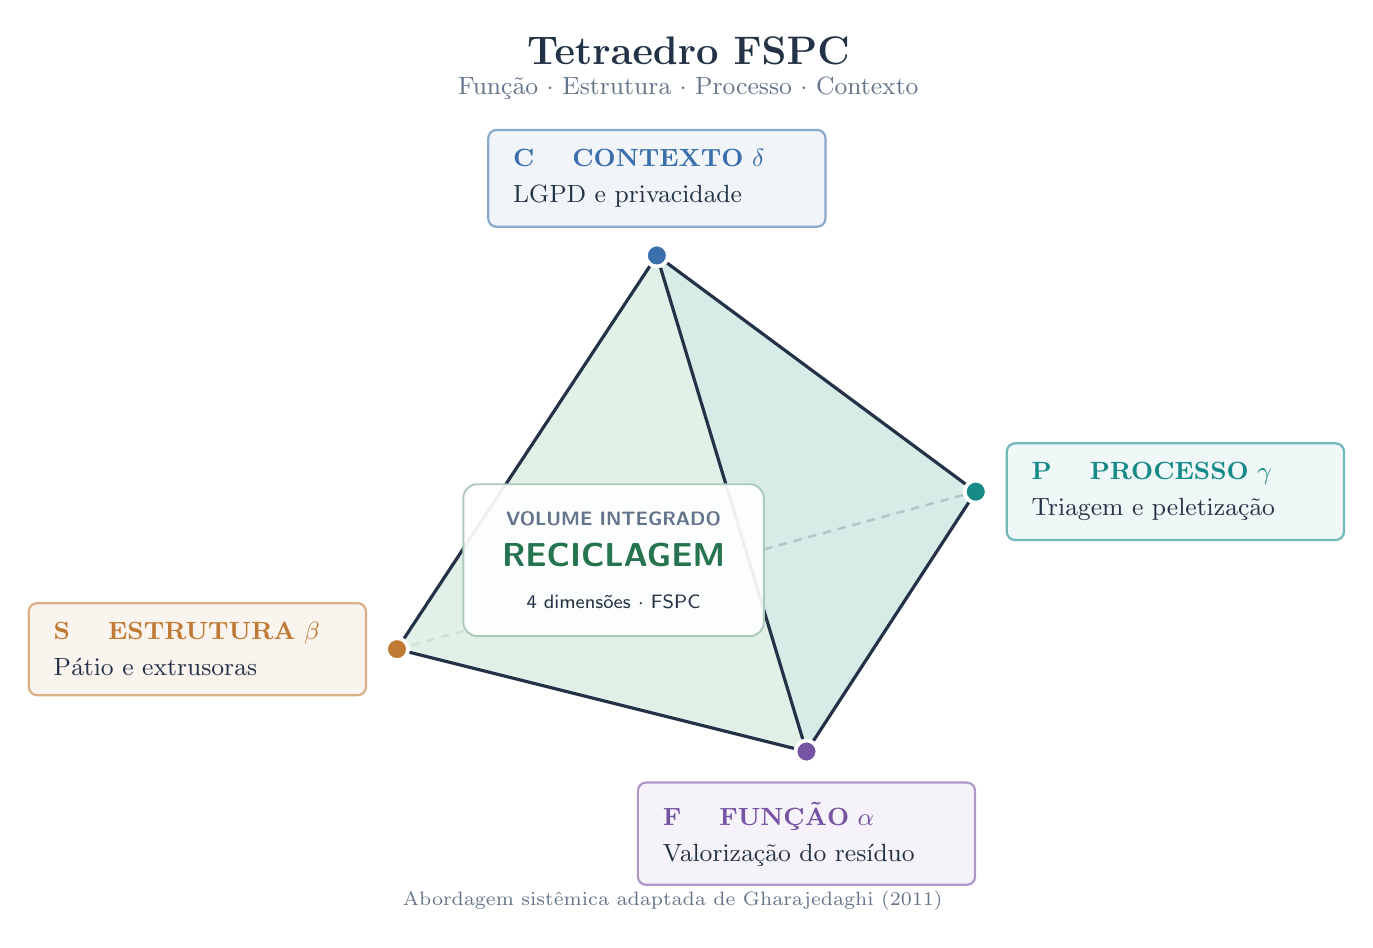
\begin{tikzpicture}[font=\sffamily]

  % Projeção: duas faces aparentes e a aresta S--P oculta.
  \coordinate (C) at (0.0,4.65);
  \coordinate (S) at (-3.30,-0.35);
  \coordinate (F) at (1.90,-1.65);
  \coordinate (P) at (4.05,1.65);

  % Cabeçalho.
  \node[font=\bfseries\Large, text=ink] at (0.4,7.25)
    {Tetraedro FSPC};
  \node[font=\small, text=muted] at (0.4,6.78)
    {Função \(\cdot\) Estrutura \(\cdot\) Processo \(\cdot\) Contexto};

  % Aresta posterior primeiro; faces translúcidas sugerem o volume.
  \draw[hidden edge] (S) -- (P);
  \fill[faceside, opacity=0.75] (C) -- (F) -- (P) -- cycle;
  \fill[facefront, opacity=0.88] (C) -- (S) -- (F) -- cycle;

  % Contorno e divisão das faces aparentes.
  \draw[edge] (C) -- (S) -- (F) -- (P) -- cycle;
  \draw[edge] (C) -- (F);

  % O resultado integrado fica dentro do sólido, sem confundir face e volume.
  \node[
    rounded corners=5pt, fill=white, fill opacity=0.93,
    text opacity=1, draw=volume!38, line width=0.7pt,
    inner xsep=14pt, inner ysep=10pt, align=center
  ] at (-0.55,0.78) {%
    {\scriptsize\bfseries\color{muted} VOLUME INTEGRADO}\\[3pt]
    {\large\bfseries\color{volume} RECICLAGEM}\\[3pt]
    {\scriptsize\color{ink} 4 dimensões \(\cdot\) FSPC}%
  };

  % Vértices, com cor e letra redundantes para leitura em escala de cinza.
  \node[vertex, fill=con] at (C) {};
  \node[vertex, fill=str] at (S) {};
  \node[vertex, fill=fun] at (F) {};
  \node[vertex, fill=pro] at (P) {};

  % Cartões externos deixam arestas e conteúdo centrais desobstruídos.
  \node[label box, draw=con!60, fill=con!7, anchor=south]
    at ($(C)+(0,0.35)$)
    {{\bfseries\color{con} C \quad CONTEXTO \(\delta\)}\\[2pt]
     {\color{ink} LGPD e privacidade}};

  \node[label box, draw=str!60, fill=str!8, anchor=east]
    at ($(S)+(-0.38,0)$)
    {{\bfseries\color{str} S \quad ESTRUTURA \(\beta\)}\\[2pt]
     {\color{ink} Pátio e extrusoras}};

  \node[label box, draw=fun!60, fill=fun!7, anchor=north]
    at ($(F)+(0,-0.38)$)
    {{\bfseries\color{fun} F \quad FUNÇÃO \(\alpha\)}\\[2pt]
     {\color{ink} Valorização do resíduo}};

  \node[label box, draw=pro!60, fill=pro!7, anchor=west]
    at ($(P)+(0.38,0)$)
    {{\bfseries\color{pro} P \quad PROCESSO \(\gamma\)}\\[2pt]
     {\color{ink} Triagem e peletização}};

  \node[font=\scriptsize, text=muted, anchor=west]
    at (-3.35,-3.55) {Abordagem sistêmica adaptada de Gharajedaghi (2011)};

\end{tikzpicture}
\end{document}
